\section{Results and Discussion}
\label{res}
%Need to explain the experimental set up here. Omnidirectional camera, monarch platform. And motivating the experiments below. 
%\dv{Need to identify one or two scenarios where the uncertainity will help us. Like two people standing close by and the robot not going in between them. In the other case with deterministic tracker, the robot should go in between them.}\\

For each of the scenarios described in section \ref{sec:scenarios}, we have compared the results obtained from the basic navigation (BN), deterministic (DHA), K-means clustering (KHA), mean shift clustering (SHA), and social cost convolution (CHA) human-aware (HA) navigation. We will only report the trajectories and metrics obtained from the results of our real experiments for the sake of conciseness. Larger values for $m_{1}$, and smaller values for $m_{2}$-$m_{5}$ are preferable.


\begin{figure}
\centering
{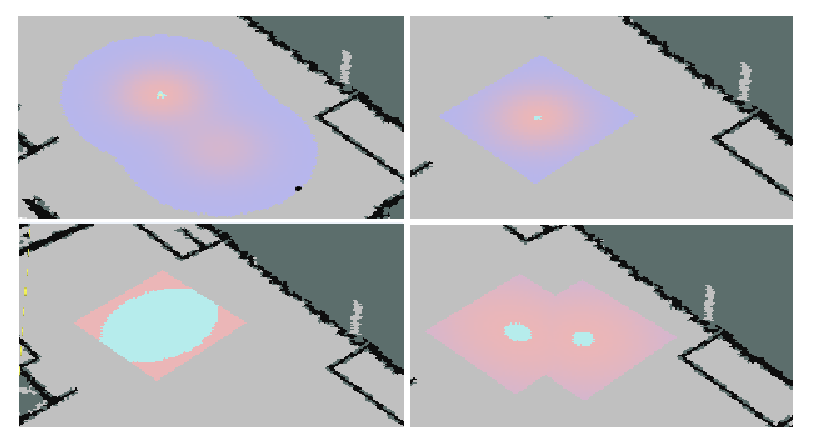
\includegraphics[width=0.42\textwidth]{pictures/all.eps}\label{fig:costmapPic}}%

\caption{Sample costmap shapes. Top right: standard 2D Gaussian, top left: Convolution method, bottom right: mean shift and bottom left: K-means.}
\label{fig:costmapPic}
\end{figure}

%1. FMM + without uncertainity\\2. FMM + with uncertainity\\	2a. Convolution\\	2b. clustering\\3. DWA + without uncertainity\\4. DWA + with uncertainity\\	2a. Convolution\\	2b. clustering\\

%All these should have simulations and real robot experiments.\\
\begin{figure}
%\left
\subfloat[]{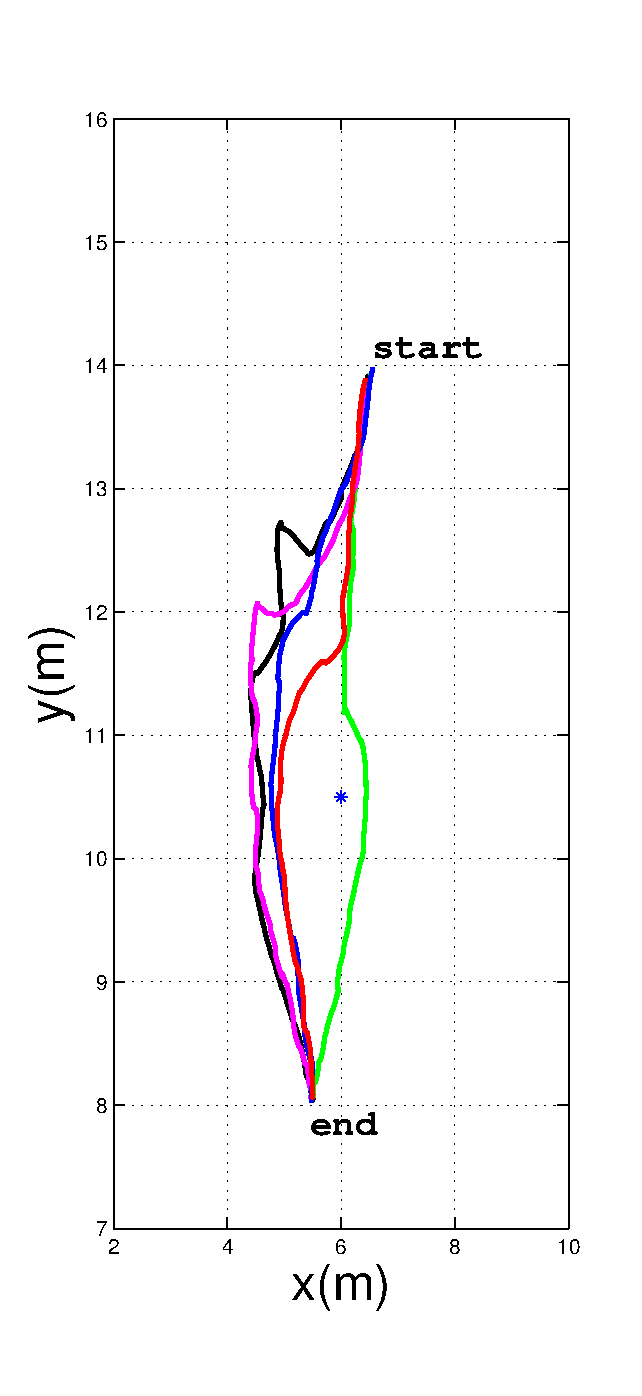
\includegraphics[width=0.17\textwidth, trim= 3mm 12.5mm 0mm 17.05mm, clip]{pictures/traj1.eps}\label{fig:traj1}}%
%\hspace{0.1cm}
\subfloat[]{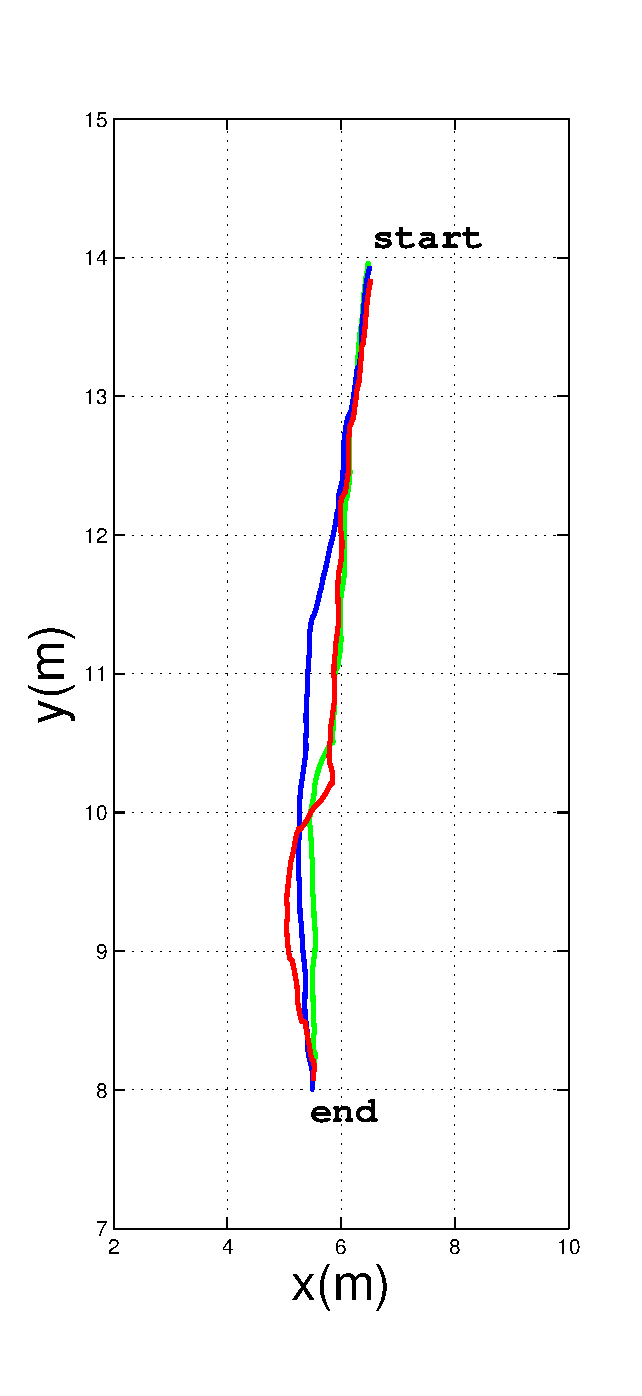
\includegraphics[width=0.17\textwidth, trim= 3mm 12.5mm 0mm 17.05mm, clip]{pictures/traj2.eps}\label{fig:traj2}}%
%\hspace{0.1cm}
\subfloat[]{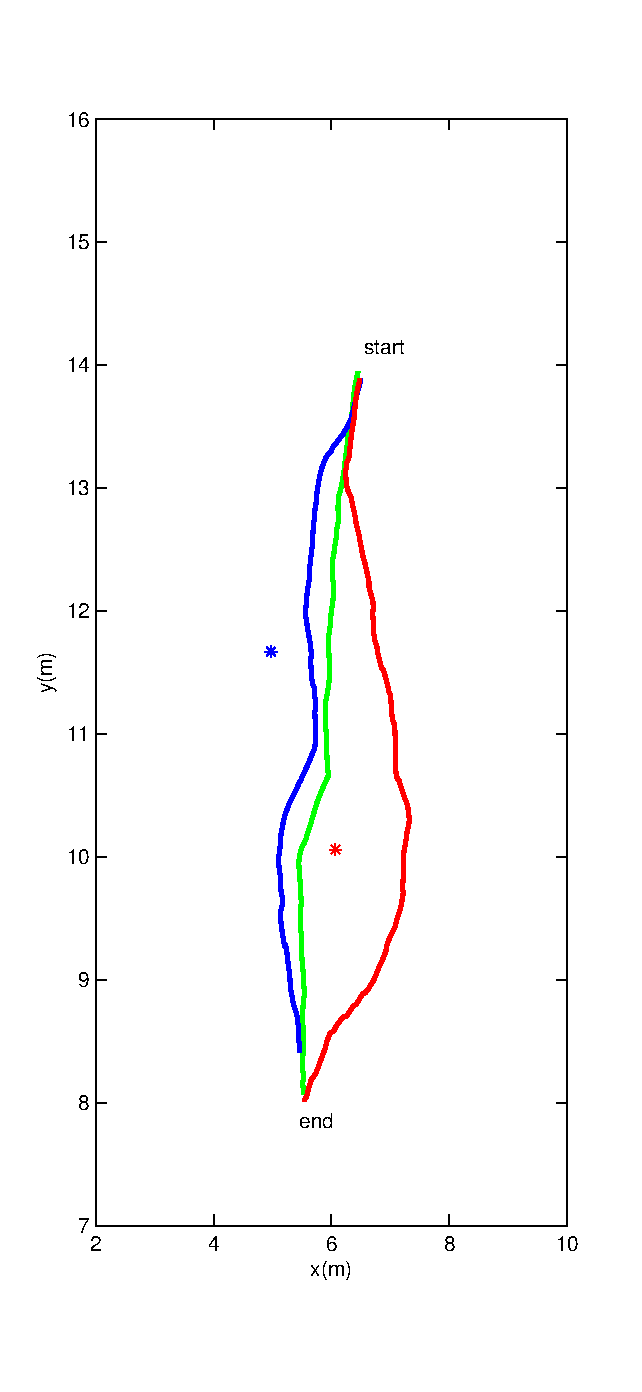
\includegraphics[width=0.17\textwidth, trim= 3mm 12.5mm 0mm 17.05mm, clip]{pictures/traj3.eps}\label{fig:traj3}}%
%\hspace{0.1cm}

\caption{Sample robot trajectories for different methods. Color coding: green for BN, red for DHA, black for KHA, pink for SHA and blue for CHA. Scenarios: (a) Single static person. (b) Single dynamic person. The person starts moving from the end point to the starting point of the robot's trajectory indicated by labels on the plots. (c) Two static people.
%Dots: static people.
}
\label{fig:trajs}
\end{figure}

\begin{figure*}
\centering
\subfloat[]{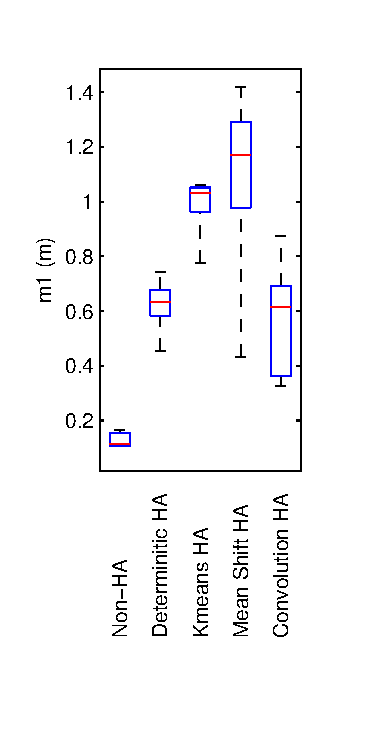
\includegraphics[width=0.175\textwidth, trim= 0mm 13mm 2mm 8mm, clip]{pictures/m1.eps}\label{fig:1_1}}%
%\hspace{%0.1cm}
\subfloat[]{\includegraphics[width=0.175\textwidth, trim= 0mm 13mm 2mm 8mm, clip]{pictures/m2.eps}\label{fig:1_2}}%
%\hspace{0.1cm}
\subfloat[]{\includegraphics[width=0.175\textwidth, trim= 0mm 13mm 2mm 8mm, clip]{pictures/m3.eps}\label{fig:1_3}}%
%\hspace{0.1cm}
\subfloat[]{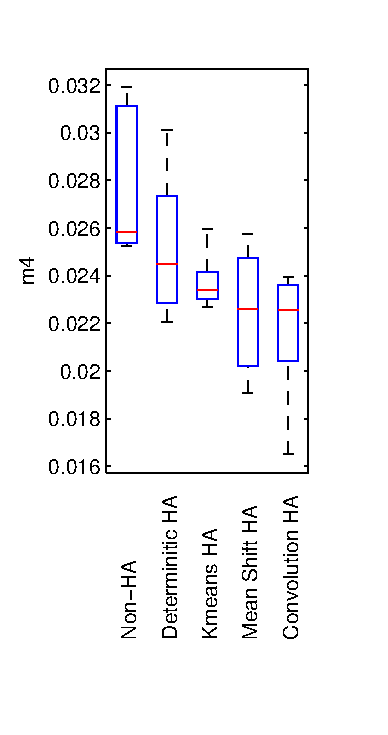
\includegraphics[width=0.175\textwidth, trim= 0mm 13mm 2mm 8mm, clip]{pictures/m4.eps}\label{fig:1_4}}%
%\hspace{0.1cm}
\subfloat[]{\includegraphics[width=0.175\textwidth, trim= 0mm 13mm 2mm 8mm, clip]{pictures/m5.eps}\label{fig:1_5}}%

\caption{Performance metrics obtained in the single static person scenario. HA stands for Human-Aware in the plot labels.
}
\label{fig:boxplots_singlePerson}
\end{figure*}

\subsection{Results}
\label{sec:results}
Figure \ref{fig:costmapPic} shows sample costmaps of the different methods mentioned earlier. It can be seen that the clustering methods can end up with saturated costs when the uncertainty is high due to large $\sigma$ values. The convolution costmap has a much more flexible shape and is not limited whereas other costmaps all have a cut off distance.

Sample trajectories of the robot are depicted in Fig. \ref{fig:trajs}. It is clear from the plots that HA methods result in trajectories that preserve larger distances to the people. Additionally, they are smoother and therefore more natural from the point of view of a person, this is supported by Fig. \ref{fig:1_4}, \ref{fig:2_2}, and \ref{fig:3_4}. However, this may not be evident from the trajectory plots. This is due to the abrupt movement of non-HA navigation upon encountering a person which considerably affects the smoothness. 

Clustering methods can cause the robot to modify its plan largely by enforcing a certain cluster shape upon finding cluster centroids: if the new probabilistic data leads to a new centroid that is not very close to the previous one, the costmap could change significantly and therefore the planned path. This is more severe for mean shift clustering due to adaptively modifying the number of clusters as well. This is to be expected given the probabilistic nature of the perception data, however the plan can be modified more smoothly using the convolution method. This method which outperforms all other methods in terms of smoothness in all of our tests, is shown to be a remedy to this problem based on our experimental results. Hence, for the second and third scenario, we only compare the results of 1) BN, 2) DHA, and 3) CHA methods.  

When comparing the results of DHA with CHA we can see that the former is a more conservative method in terms of keeping distance to the people when receiving accurate data. If DHA receives a perfect estimate of the person's position it can lead to the desired path, however this is seldom the case. Particularly, in the case of a moving person, the detector could not always keep up with the speed of the person, \textit{i.e.}, the position estimates were reported with delay or the person was lost in some cases, and the robot was faced with the human while considering him an obstacle. This led to abrupt changes and getting too close to the person, see Fig.~\ref{fig:traj2}. However, CHA by associating larger uncertainty to the estimates in this case, could lead to better plans in terms of proximity and smoothness. Unfortunately, due to our inaccurate ground truth of the moving person, we only rely on $m_{4}$ and $m_{5}$ for scenario 2, but we observed the delayed perception and lost person problem during our experiments. 




\begin{figure}[!]
\centering
\subfloat[]{\includegraphics[width=0.150\textwidth, trim= 0mm 13mm 2mm 8mm, clip]{pictures/dy_m4.eps}\label{fig:2_2}}%
\hspace{0.1cm}
\subfloat[]{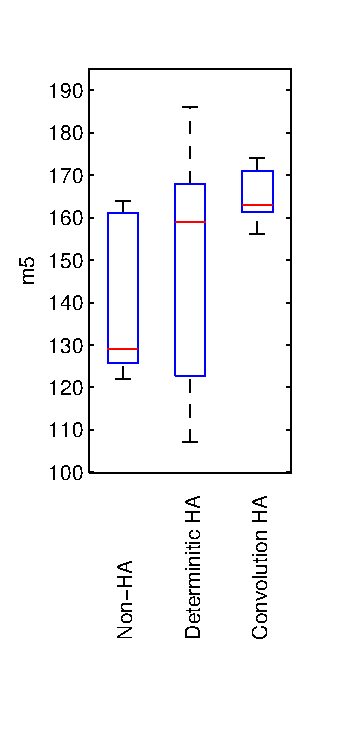
\includegraphics[width=0.15\textwidth, trim= 0mm 13mm 2mm 8mm, clip]{pictures/dy_m5.eps}\label{fig:2_3}}%

\caption{Performance metrics obtained in the dynamic person scenario. %HA stands for Human-Aware in the plot labels.
}
\label{fig:boxplots_singlePersonMov}
\end{figure}

%
\begin{figure}[t!]
\centering
\subfloat[]{\includegraphics[width=0.164\textwidth, trim= 2mm 13mm 2mm 9mm, clip ]{pictures/two_m1.eps}\label{fig:3_1}}% \vspace{<whatever>}
%\hspace{0.1cm}
\subfloat[]{\includegraphics[width=0.164\textwidth, trim= 2mm 13mm 2mm 9mm, clip ]{pictures/two_m2.eps}\label{fig:3_2}}%
%\hspace{0.1cm}
\subfloat[]{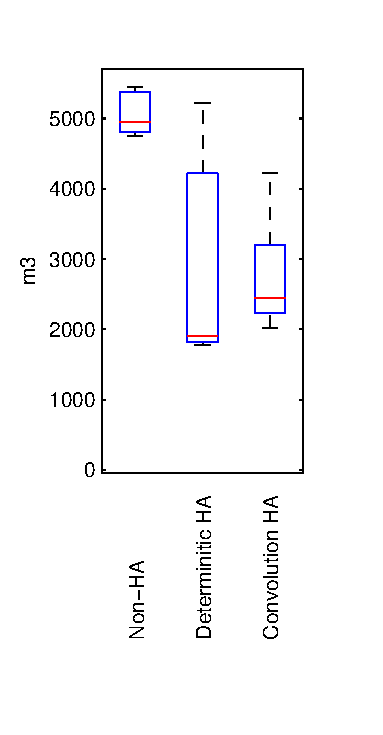
\includegraphics[width=0.164\textwidth, trim= 2mm 13mm 2mm 9mm, clip ]{pictures/two_m3.eps}\label{fig:3_3}}%

%\hspace{0.1cm}
\subfloat[]{\includegraphics[width=0.164\textwidth, trim= 2mm 13mm 2mm 9mm, clip ]{pictures/two_m4.eps}\label{fig:3_4}}%
%\hspace{0.1cm}
\subfloat[]{\includegraphics[width=0.164\textwidth, trim= 2mm 13mm 2mm 9mm, clip ]{pictures/two_m5.eps}\label{fig:3_5}}%
%\hspace{0.1cm}
%\subfloat[]{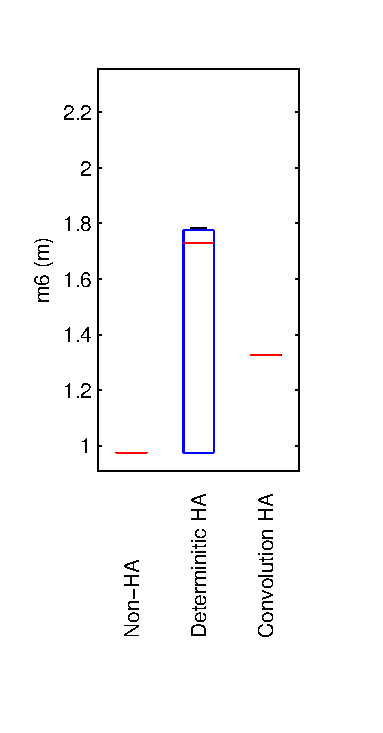
\includegraphics[width=0.163\textwidth, trim= 2mm 13mm 2mm 8mm, clip ]{pictures/two_m6.eps}\label{fig:3_6}}%

\caption{Performance metrics obtained in the two static people scenario.
% HA stands for Human-Aware in the plot labels.
}
\label{fig:boxplots_2people}
\end{figure}


Figures \ref{fig:boxplots_singlePerson}, \ref{fig:boxplots_singlePersonMov} and \ref{fig:boxplots_2people} show the performance metrics for the three scenarios. We will discuss the results of each metric in the following. $m_{1}$ has increased for HA methods which shows the effectiveness of our FMM planner in social path planning. However, DHA is more conservative in this regard in the presence of good perception data. $m_{2}$ has increased for uncertainty-based methods in the simple scenario as the deterministic tracker is giving already good position estimates, but this is no longer the case when the complexity is increased as seen in Fig. \ref{fig:3_2}. $m_{3}$ is also reduced for HA methods and more so for uncertainty-based HA methods as the complexity of the problem increases, see Fig.\ref {fig:3_3}.


$m_{4}$ is showing a very interesting result, we can see how uncertainty-based HA methods have managed to introduce smoothness into the trajectories by reducing jerk without deliberately accounting for it. CHA is dominating other methods across all scenarios in this case. Lastly, $m_{5}$ which shows the total navigation time is always lower for BN due to optimizing the path length only. The largest values belong to KHA and SHA due to constant modifications of the path, thus taking longer routes. For DHA this metric is lower than CHA for the static person case and comparable to CHA in the moving person scenario, but it increases as the complexity of the environment grows further in the case of multiple people.% Lastly, $m_{6}$ which is only used in the third scenario, indicates how DHA has varying behavior (sometimes takes a detour) based on the tracker estimates whereas CHA has more or less the same behavior in our runs due to its probabilistic nature when computing the social costmap.     



%\subsection{Discussion}
%\label{sec:discussion}
